\documentclass[12pt,]{article}
\usepackage{lmodern}
\usepackage{amssymb,amsmath}
\usepackage{ifxetex,ifluatex}
\usepackage{fixltx2e} % provides \textsubscript
\ifnum 0\ifxetex 1\fi\ifluatex 1\fi=0 % if pdftex
  \usepackage[T1]{fontenc}
  \usepackage[utf8]{inputenc}
\else % if luatex or xelatex
  \ifxetex
    \usepackage{mathspec}
  \else
    \usepackage{fontspec}
  \fi
  \defaultfontfeatures{Ligatures=TeX,Scale=MatchLowercase}
    \setmainfont[]{Times New Roman}
\fi
% use upquote if available, for straight quotes in verbatim environments
\IfFileExists{upquote.sty}{\usepackage{upquote}}{}
% use microtype if available
\IfFileExists{microtype.sty}{%
\usepackage{microtype}
\UseMicrotypeSet[protrusion]{basicmath} % disable protrusion for tt fonts
}{}
\usepackage[margin=2.54cm]{geometry}
\usepackage{hyperref}
\hypersetup{unicode=true,
            pdftitle={Examining the Relationship between Flow and Nutrient Levels at Upstream and Downstream Locations along Ellerbe Creek, North Carolina},
            pdfauthor={Rachel Landman},
            pdfborder={0 0 0},
            breaklinks=true}
\urlstyle{same}  % don't use monospace font for urls
\usepackage{longtable,booktabs}
\usepackage{graphicx,grffile}
\makeatletter
\def\maxwidth{\ifdim\Gin@nat@width>\linewidth\linewidth\else\Gin@nat@width\fi}
\def\maxheight{\ifdim\Gin@nat@height>\textheight\textheight\else\Gin@nat@height\fi}
\makeatother
% Scale images if necessary, so that they will not overflow the page
% margins by default, and it is still possible to overwrite the defaults
% using explicit options in \includegraphics[width, height, ...]{}
\setkeys{Gin}{width=\maxwidth,height=\maxheight,keepaspectratio}
\IfFileExists{parskip.sty}{%
\usepackage{parskip}
}{% else
\setlength{\parindent}{0pt}
\setlength{\parskip}{6pt plus 2pt minus 1pt}
}
\setlength{\emergencystretch}{3em}  % prevent overfull lines
\providecommand{\tightlist}{%
  \setlength{\itemsep}{0pt}\setlength{\parskip}{0pt}}
\setcounter{secnumdepth}{5}
% Redefines (sub)paragraphs to behave more like sections
\ifx\paragraph\undefined\else
\let\oldparagraph\paragraph
\renewcommand{\paragraph}[1]{\oldparagraph{#1}\mbox{}}
\fi
\ifx\subparagraph\undefined\else
\let\oldsubparagraph\subparagraph
\renewcommand{\subparagraph}[1]{\oldsubparagraph{#1}\mbox{}}
\fi

%%% Use protect on footnotes to avoid problems with footnotes in titles
\let\rmarkdownfootnote\footnote%
\def\footnote{\protect\rmarkdownfootnote}

%%% Change title format to be more compact
\usepackage{titling}

% Create subtitle command for use in maketitle
\providecommand{\subtitle}[1]{
  \posttitle{
    \begin{center}\large#1\end{center}
    }
}

\setlength{\droptitle}{-2em}

  \title{Examining the Relationship between Flow and Nutrient Levels at Upstream
and Downstream Locations along Ellerbe Creek, North Carolina}
    \pretitle{\vspace{\droptitle}\centering\huge}
  \posttitle{\par}
  \subtitle{\url{https://github.com/rml41/EDA_2020_Project.git}}
  \author{Rachel Landman}
    \preauthor{\centering\large\emph}
  \postauthor{\par}
    \date{}
    \predate{}\postdate{}
  
\usepackage{float}

\begin{document}
\maketitle

\newpage
\tableofcontents 
\newpage
\listoftables 
\newpage
\listoffigures 
\newpage

\hypertarget{rationale-and-research-questions}{%
\section{Rationale and Research
Questions}\label{rationale-and-research-questions}}

Ellerbe Creek runs through the city of Durham, North Carolina into the
Falls Lake Resevoir. Falls Lake serves as the source of drinking water
for the City of Raleigh and does not meet North Carolina standards for
\emph{chlorophyll a}, which is found in algae (City of Durham, 2020).
Algal blooms that lead to increased \emph{chlorophyll a} generally come
from excess nutrients such as phosphorus and nitrogen. Ellerbe Creek is
one of the sources of excess nutrients and contaminents in Falls Lake.
The Ellerbe Creek Watershed has the highest population density of
Durham's watersheds, with an estimated 22\% impervious surface (NC DEQ,
2009). It is impacted by both point and nonpoint sources and was found
to deliver the highest nutrient loads to Falls Lake (NC DEQ, 2009).
Ellerbe Creek and Falls Lake are both on the state's impaired water
bodies list (303(d) list) (City of Durham, 2018). Ellerbe Creek was
first listed on the 303(d) list in 1998 (NC DEQ, 2009). While Ellerbe
Creek and Falls Lake have been on the state's impaired water bodies
list, there is still excess nitrogen and phosphorus leading to
\emph{chlorophyll a} in Falls Lake. In order to achieve nitrogen and
phosphorus reductions it is important to understand when nutrient levels
are highest and what factors influence high concentrations. This
information will help managers determine the best managment practices
for nitrogen and phosphorus removal. This dataset was chosen because it
compiles nitrogen and phosphorus data from monitoring locations along
Ellerbe Creek allowing for analysis of the entire watershed. It was
matched with USGS discharge data from two sites to examine the
differences between upstream and downstream locations.

\textbf{This analysis and report will aim to answer the following
questions:}

\begin{enumerate}
\def\labelenumi{\arabic{enumi}.}
\item
  Are nitrogen and phosphorus levels in Ellerbe Creek above recommended
  levels?
\item
  Is there a relationship between flow and nitrogen or phosphorus
  concentrations?
\item
  How does location, upstream vs.~downstream, impact nutrient levels?
\item
  Is there a significant difference between discharge at the upstream
  and downstream gages?
\item
  Is time of year, specifically month a predictor of flow or nutrient
  levels?
\end{enumerate}

\newpage

\hypertarget{dataset-information}{%
\section{Dataset Information}\label{dataset-information}}

Nutrient data for this project were downloaded from the the Water
Quality Portal, a coorperative service sponsered by the United States
Geological Survey (USGS), the Environmental Protection Agency (EPA), and
the National Water Quality Monitoring Council (NWQMC) on February 27,
2020. Discharge data were downloaded for two stream gages along Ellerbe
Creek, HUC code 030202010403, from USGS using the data dataRetrieval
package in R. The dataset analyzed contains 21 monitoring locations with
measurments for nitrogen and phosphorus levels from 1982 to 2018 and
daily discharge data from 2008 to 2020. Not all locations had data for
each nutrient. Nitrogen and phosphorus concentrations are recorded as
mg/L of nitrogen or phosphorus in various compounds including, nitrate,
nitrite, ammonia, ammonium, organic nitrogen, phosphate, and organic
phosphorus. The USGS gage locations are Club Blvd (0208675010),
upstream, and Gorman (02086849), downstream.

Table 1. Variables Analyzed from the Water Quality and USGS Gage
Datasets

\begin{longtable}[]{@{}llllll@{}}
\toprule
Variable & Units & Range & Mean & Median & Source\tabularnewline
\midrule
\endhead
Nitrogen & mg/L N & 0.37 - 33.00 & 7.18 & 2.82 & NC DENR and
USGS\tabularnewline
Phosphorus & mg/L P & 0.039 - 17.00 & 1.091 & 0.157 & NC DENR and
USGS\tabularnewline
Discarge Club & ft\textsuperscript{3}/s & 0.20 - 781.00 & 9.39 & 1.28 &
USGS\tabularnewline
Discharge Gorman & ft\textsuperscript{3}/s & 7.52 - 1750.00 & 48.84 &
20.50 & USGS\tabularnewline
\bottomrule
\end{longtable}

\hypertarget{discharge-data-wrangling}{%
\subsection{Discharge Data Wrangling}\label{discharge-data-wrangling}}

Flow data from the two USGS stream gages were combined into two
datasets, one as a long format with all discharge in one column and one
in wide format, with two seperate columns for discharge based on
location.

\hypertarget{nutrient-data-wrangling}{%
\subsection{Nutrient Data Wrangling}\label{nutrient-data-wrangling}}

The nutrient dataset from the water quality portal was cleaned to remove
all irrelevant information and retain just characteristics of interest,
nitrogen and phosphorus. Nitrogen and phosphorus values for many samples
were recorded as both mg/L of N and P, and of NO3 and PO4 respectively.
Data were downloaded in long format and were converted to wide format in
order to convert nitrogen and phosphorus values to mg/L of N or P.
Relevant columns such as data, location, hydrologic event, variable
name, measured value, and units were selected and processed data were
saved as both long and wide format.

\newpage

\hypertarget{exploratory-analysis}{%
\section{Exploratory Analysis}\label{exploratory-analysis}}

\hypertarget{initial-exploration}{%
\subsection{Initial Exploration}\label{initial-exploration}}

Explored raw data from the water quality portal to determine potential
variables for analysis and time period of data. Examined a summary of
all the characteristics in the dataset to determine the count for each
variable. Selected Nitrogen, mixed forms (NH3), (NH4), organic, (NO2)
and (NO3) and Phosphorus as the two variables to analyze. Explored
discharge data to determine date range of data.

Table 2. Sample of summary results from raw data

\begin{longtable}[]{@{}ll@{}}
\toprule
Variable & Count\tabularnewline
\midrule
\endhead
Dissolved Oxygen & 636\tabularnewline
Nitrate & 128\tabularnewline
Nitrogen, mixed forms (NH3), (NH4), organic, (NO2) and (NO3) &
209\tabularnewline
Phosphorus & 286\tabularnewline
RBP Stream Width & 14\tabularnewline
Temperature, water & 1146\tabularnewline
Total Dissolved Solids & 278\tabularnewline
\bottomrule
\end{longtable}

\hypertarget{location-of-monitoring-sites}{%
\subsection{Location of Monitoring
Sites}\label{location-of-monitoring-sites}}

Monitoring sites were maped to determine their locations within the
Ellere Creek Watershed and their proximity to Falls Lake (Fig. 1).
Monitoring sites represent the location of Ellerbe Creek and show its
flow through the watershed. The map was used to determine which sites to
classify as upstream and which to classify as downstream.

\begin{figure}
\centering
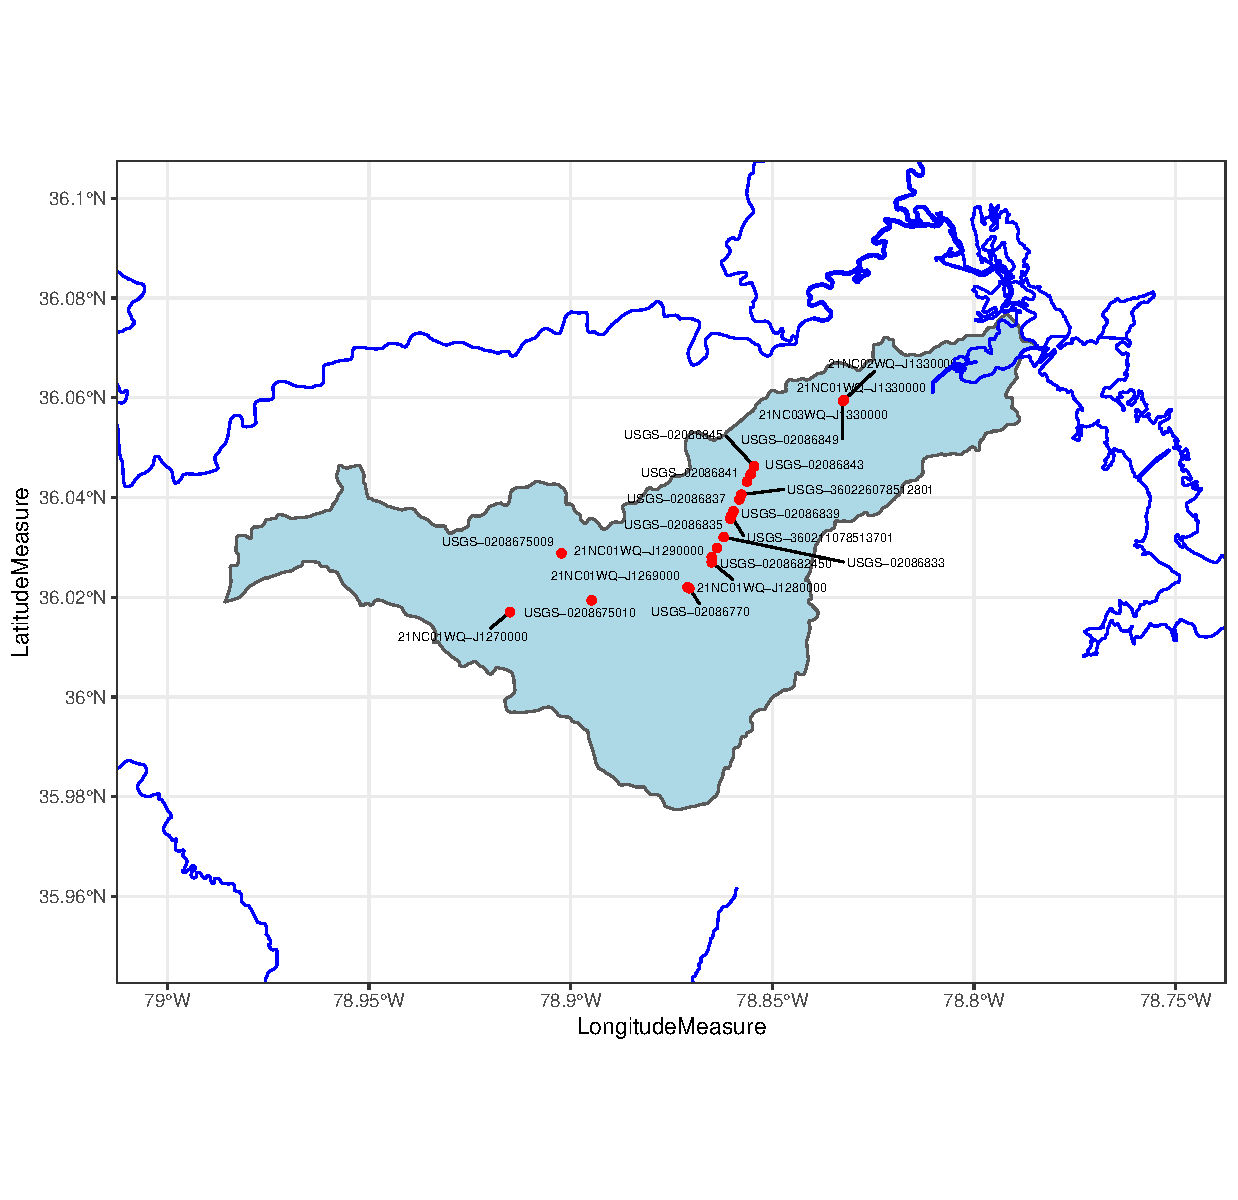
\includegraphics{Landman_ENV872_Project_files/figure-latex/Exploratory Analysis Figure 1-1.pdf}
\caption{Map of the Ellerbe Creek Watershed and Monitoring Locations
along Ellerbe Creek Ranked from Upstream to Downstream}
\end{figure}

\newpage

\hypertarget{discharge-data-exploration}{%
\subsection{Discharge Data
Exploration}\label{discharge-data-exploration}}

A boxplot was made to visualize the range of discharge at each site
(Fig. 2). The distribution shows that the max discharge from 2008-2020
is higher at the downstream location (2086849) than the upstream
location (208675010), but it is not obvious if the mean is different.
This led to running statistical analysis to determine if the difference
in average discharge is significant. If there is a significant
difference in discharge between upstream and downstream, that could
influence the nutrient levels at each site.

\begin{figure}
\centering
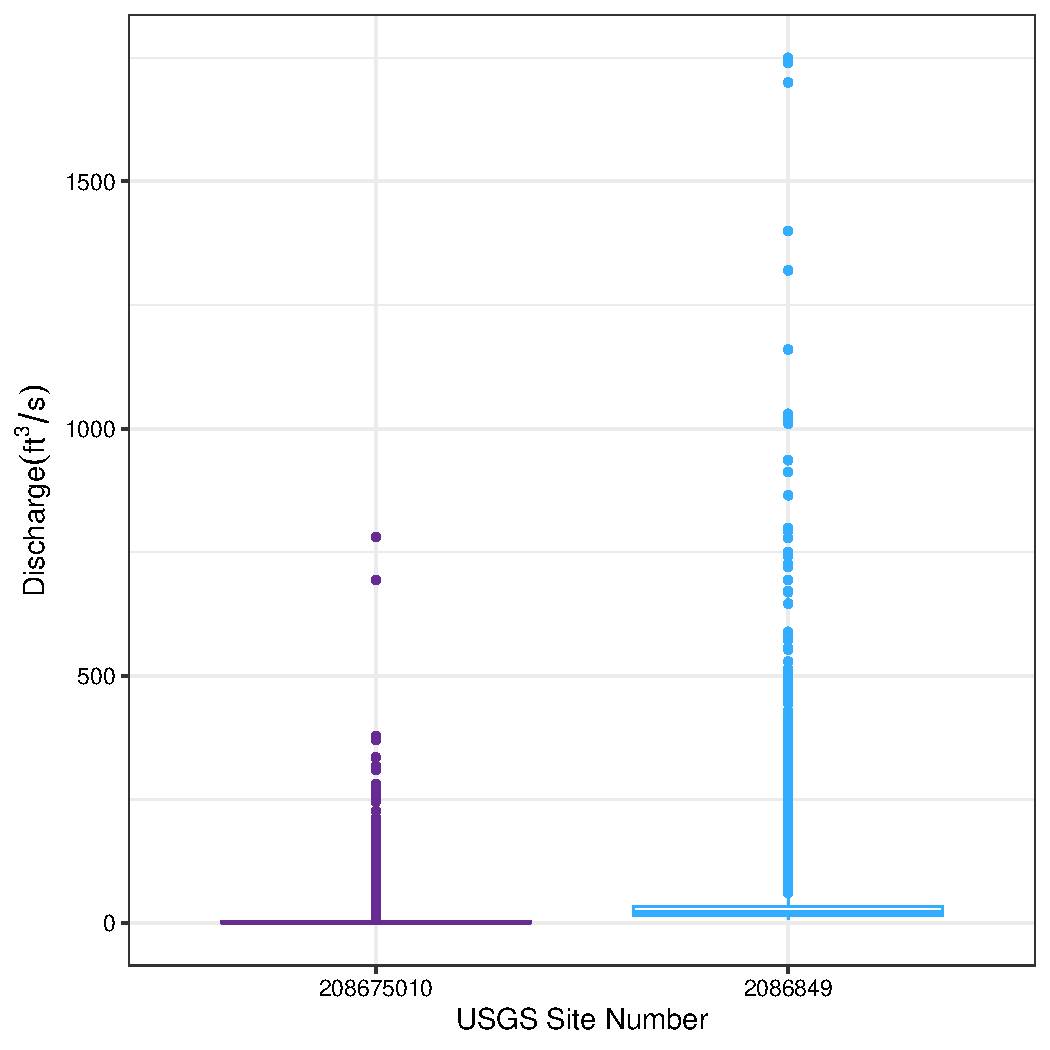
\includegraphics{Landman_ENV872_Project_files/figure-latex/Exploratory Analysis Figure 2-1.pdf}
\caption{Distribution of discharge at two sites, upstream (208675010)
and downstream (2086849) along Ellerbe Creek from January 1, 2008 to
April 17, 2020}
\end{figure}

\newpage

The discharge over time at each location does not show any obvious
seasonal or annual trends (Fig. 3).

\begin{figure}
\centering
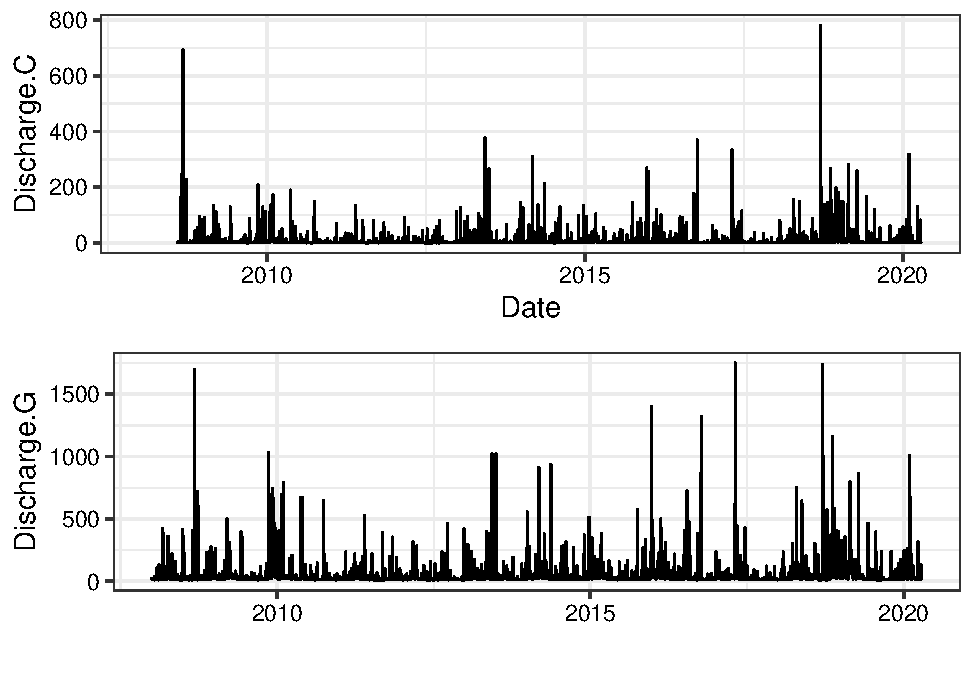
\includegraphics{Landman_ENV872_Project_files/figure-latex/Exploratory Analysis Figure 3-1.pdf}
\caption{Daily discharge (Q) along Ellerbe Creek from January 1, 2008 to
April 17, 2020}
\end{figure}

\newpage

\hypertarget{nutrient-data-exploration}{%
\subsection{Nutrient Data Exploration}\label{nutrient-data-exploration}}

The distribution of the nitrogen and phosphorus concentrations shows
that the mean and max nitrogen concetrations look higher than those for
phosphorus (Fig. 4). Statistical analysis will determine if there is a
significant difference in the concentrations of each nutrient. The range
for nitrogen is very wide and therefore it will be interesting to
examine potential causes for high and low concentrations.

\begin{figure}
\centering
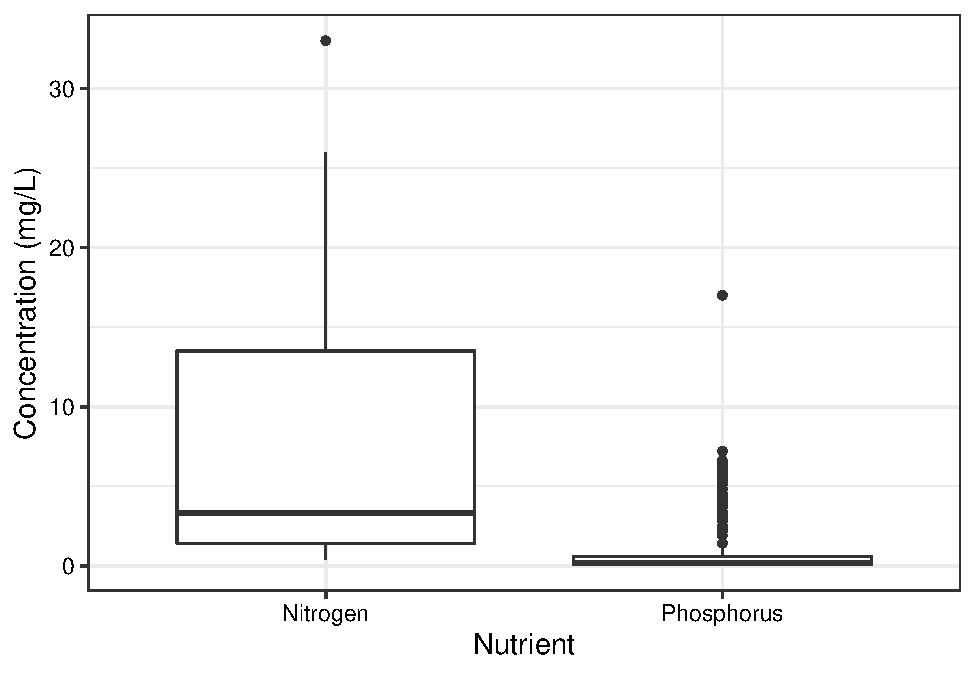
\includegraphics{Landman_ENV872_Project_files/figure-latex/Exploratory Analysis Figure 4-1.pdf}
\caption{Distribution of Nitrogen and Phosphorus Concentrations in
Ellerbe Creek from November 17, 1982 to December 17, 2018}
\end{figure}

It is surprising that the values for nitrogen and phosphorus
concentration have changed so drastically from the 1980s to the 2000s.
Although measurement units were converted, the concentrations in the
1980s seem to be higher and have a wider range than expected.

\begin{figure}
\centering
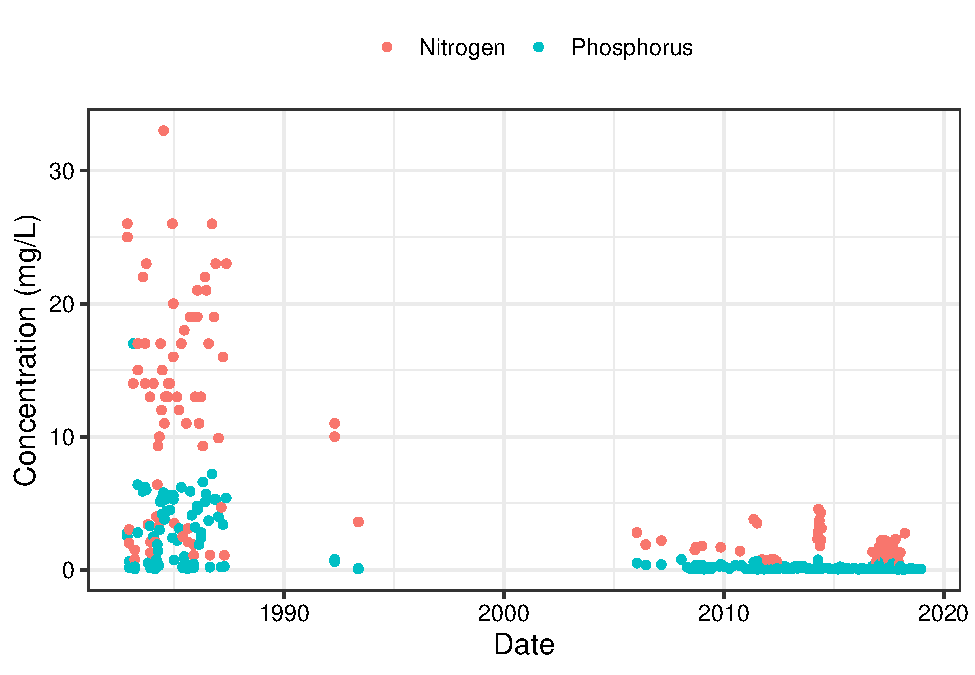
\includegraphics{Landman_ENV872_Project_files/figure-latex/Exploratory Analysis Figure 5-1.pdf}
\caption{Concentrations of Nitrogen and Phosphorus over Time in Ellerbe
Creek from November 17, 1982 to December 17, 2018}
\end{figure}

\newpage

\hypertarget{analysis}{%
\section{Analysis}\label{analysis}}

\hypertarget{question-1-are-nitrogen-and-phosphorus-levels-in-ellerbe-creek-above-recommended-levels}{%
\subsection{Question 1: Are nitrogen and phosphorus levels in Ellerbe
Creek above recommended
levels?}\label{question-1-are-nitrogen-and-phosphorus-levels-in-ellerbe-creek-above-recommended-levels}}

The maximun contaminent level (MCL) for nitrate is 10 mg/L and for
nitrite is 1 mg/L, but there is not a recommended water quality standard
for total nitrogen, which is analyzed in this report. The EPA states
that an acceptable range for total nitrogen is 2 mg/L to 6 mg/L (EPA
Nitrogen, 2013). There is no MCL for phosphorus, but the EPA says that
0.01 mg/L to 0.04 mg/L is an acceptable range (EPA Phosphorus, 2013).
The mean concentration of each nutrient was compared with the higher end
of the acceptable range to determine if nutrient levels in Ellerbe Creek
are above recommended levels. In Table 3 you can see that the mean
concentrations of N and P in the creek are both above the recommended
levels. Because the data are not normally distributed (Fig 6), a
nonparametric stastical test was run. The results indicate that the
average concentration of nitrogen in Ellerbe Creek from 1984-2008 is not
significantly greater than highest recommended value of 6 mg/L
(wilcoxon, p=0.3318). The average concentration of phosphours in Ellerbe
Creek from 1984-2008 is significantly higher than the highest
recommended value of 0.04 mg/L (wilcoxon, p=0.033). The density plot in
figure 6 shows the distribution of the data with a veritcal line
representing the maximun recommended level of each nutrient.

\begin{longtable}[]{@{}rrrrrrrr@{}}
\caption{Summary of Total Nitrogen and Phosphorus
Conentrations}\tabularnewline
\toprule
mean.N & min.N & max.N & St.dev.N & mean.P & min.P & max.P &
St.dev.P\tabularnewline
\midrule
\endfirsthead
\toprule
mean.N & min.N & max.N & St.dev.N & mean.P & min.P & max.P &
St.dev.P\tabularnewline
\midrule
\endhead
7.183095 & 0.37 & 33 & 7.773407 & 1.091398 & 0.039 & 17 &
2.082384\tabularnewline
\bottomrule
\end{longtable}

\newpage

\begin{figure}
\centering
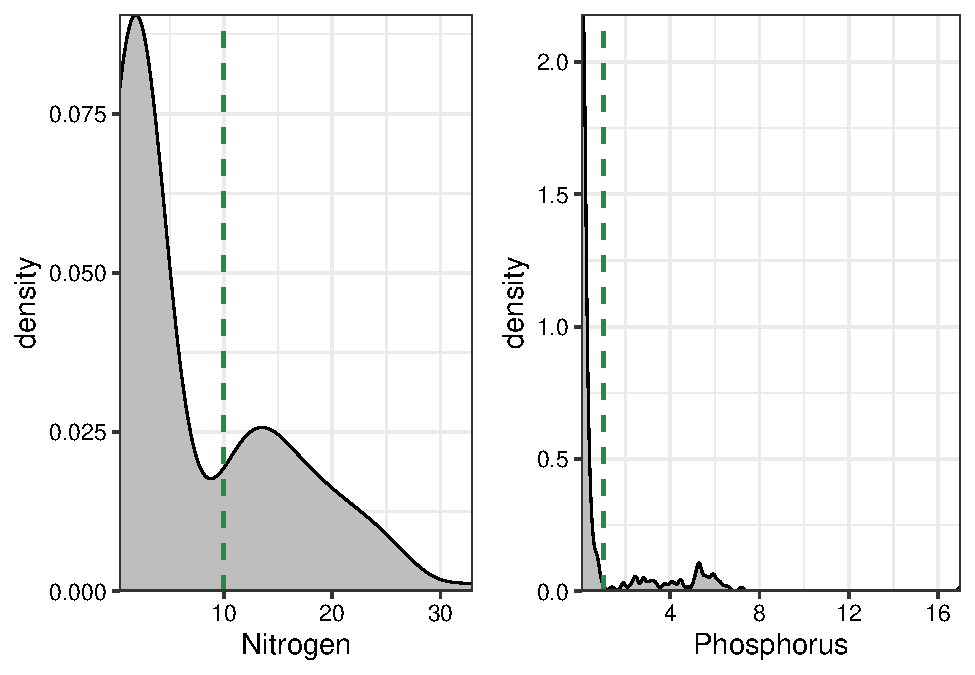
\includegraphics{Landman_ENV872_Project_files/figure-latex/Data Analysis Figure 6-1.pdf}
\caption{Density plots of Nitrogen and Phosphorus Concentrations}
\end{figure}

\newpage

\hypertarget{question-2-is-there-a-relationship-between-flow-and-nitrogen-or-phosphorus-levels}{%
\subsection{Question 2: Is there a relationship between flow and
nitrogen or phosphorus
levels?}\label{question-2-is-there-a-relationship-between-flow-and-nitrogen-or-phosphorus-levels}}

There is no significant relationship between Nitrogen and discharge at a
significance of 0.05, but there is nearly a significant relationship at
the 0.1 signifance level (Simple Linear Regression, Adj R-squared =
0.018, df = 62, p = 0.1442). While we can't conclusively say there is a
negative relationship between nitrogen concetration and flow, you can
see a downward trend in the results (Fig. 7). Flow is a significant
predictor of phosphorus levels and 33\% of the variance in phosphorus
concentration can be explained by flow in Ellerbe Creek (Simple Linear
Regression, Adj R-squared = 0.3276, df = 162, p \textless{} 0.0001). As
flow increases so does the concentration of Phosphorus (Fig. 8).

\begin{figure}
\centering
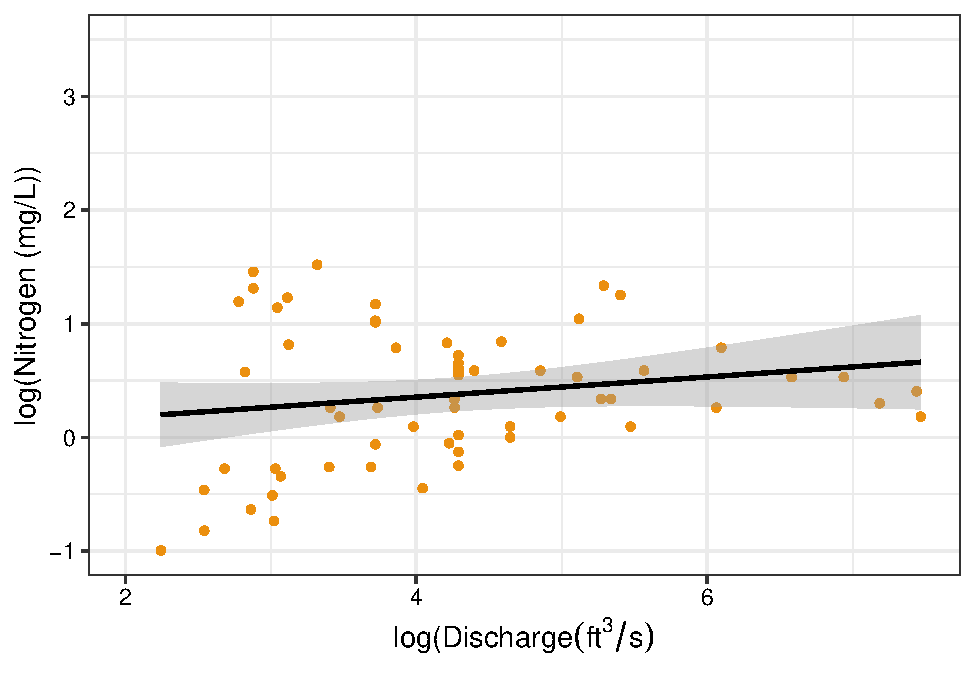
\includegraphics{Landman_ENV872_Project_files/figure-latex/Data Analysis Figure 7-1.pdf}
\caption{Linear regression of the log of Nitrogen Concentration vs.~the
log of Discharge}
\end{figure}

\begin{figure}
\centering
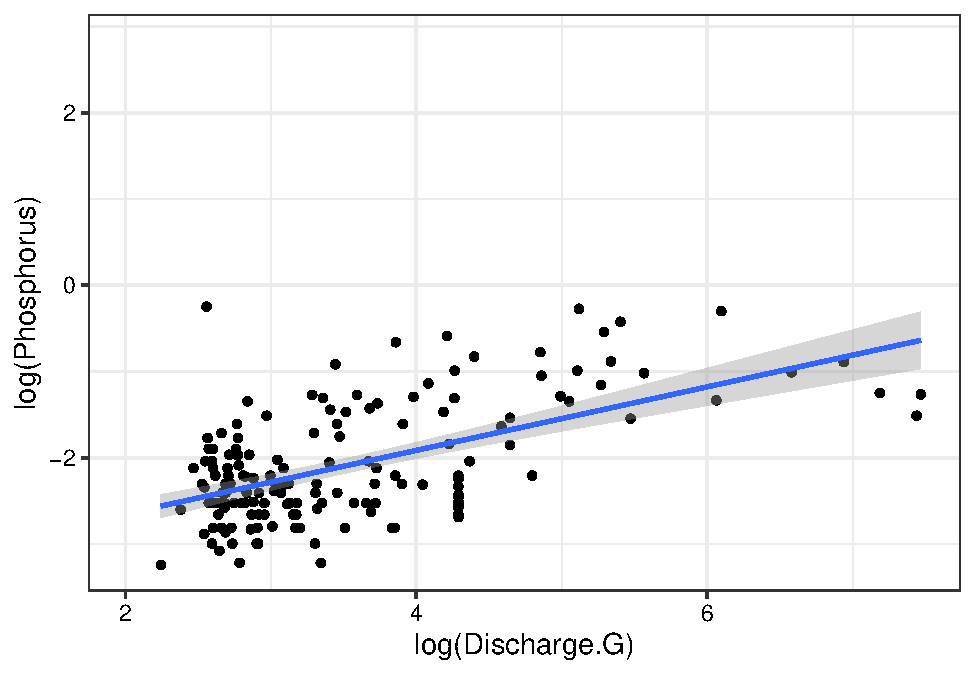
\includegraphics{Landman_ENV872_Project_files/figure-latex/Data Analysis Figure 8-1.pdf}
\caption{Linear regression of the log of Phosphorus Concentration
vs.~the log of Discharge}
\end{figure}

\newpage

\hypertarget{question-3-how-does-location-upstream-vs.downstream-impact-nutrient-levels}{%
\subsection{Question 3: How does location, upstream vs.~downstream,
impact nutrient
levels?}\label{question-3-how-does-location-upstream-vs.downstream-impact-nutrient-levels}}

The mean nitrogen concentration from 1984-2018 is significantly higher
downstream near where Ellerbe Creek enters Falls Lake than it is
upstream near Club Blvd (Wilcoxon, p \textless{} 0.0001). There is no
significant difference between the mean concentration of phosphorus at
the upstream and downstream monitoring sites (Wilcoxon, p = 0.1651)
(Fig. 9; Table 4). Higher levels of nitrogen downstream would indicate
that there is a source of nitrogen entering the creek between the two
locations.

\begin{longtable}[]{@{}lrrrrrrrr@{}}
\caption{Summary of Nitrogen and Phosphorus conentrations by
Location}\tabularnewline
\toprule
Location & mean.N & min.N & max.N & St.dev.N & mean.P & min.P & max.P &
St.P\tabularnewline
\midrule
\endfirsthead
\toprule
Location & mean.N & min.N & max.N & St.dev.N & mean.P & min.P & max.P &
St.P\tabularnewline
\midrule
\endhead
Downstream & 10.057376 & 0.79 & 33.0 & 8.0439064 & 1.300915 & 0.040 &
17.00 & 2.2616513\tabularnewline
Upstream & 1.141212 & 0.37 & 2.3 & 0.5175167 & 0.223875 & 0.039 & 0.74 &
0.1695302\tabularnewline
\bottomrule
\end{longtable}

\hypertarget{question-4-is-there-a-significant-difference-between-discharge-at-the-upstream-and-downstream-gages}{%
\subsection{Question 4: Is there a significant difference between
discharge at the upstream and downstream
gages?}\label{question-4-is-there-a-significant-difference-between-discharge-at-the-upstream-and-downstream-gages}}

Average discharge from 2008-2020 is significantly higher downstream near
where Ellerbe Creek enters Falls Lake than it is upstream (Wilcoxon,
p-value \textless{} 0.0001). There are multiple factures that could lead
to greater discharge upstream than downstream including the catchment
area. One hypothesis is there is more runoff between the two locations
which increases flow downstream.

\begin{longtable}[]{@{}lrrrr@{}}
\caption{Summary of Discharge by Location}\tabularnewline
\toprule
Location & mean.Flow & min.Flow & max.Flow &
Standard.dev.Flow\tabularnewline
\midrule
\endfirsthead
\toprule
Location & mean.Flow & min.Flow & max.Flow &
Standard.dev.Flow\tabularnewline
\midrule
\endhead
Downstream & 47.955745 & 7.52 & 1750 & 110.38991\tabularnewline
Upstream & 8.073456 & 0.02 & 781 & 29.86186\tabularnewline
\bottomrule
\end{longtable}

\hypertarget{question-5-is-time-of-year-specifically-month-a-predictor-for-flow-or-nutrient-levels}{%
\subsection{Question 5: Is time of year, specifically month a predictor
for flow or nutrient
levels?}\label{question-5-is-time-of-year-specifically-month-a-predictor-for-flow-or-nutrient-levels}}

Because there is a significant relationship between flow and phosphorus
levels, it is interesting to examine if there are seasonal trends in
that relationship. Month is a significant predictor of flow, which makes
sense because precipitation and runoff change between seasons
(Kruskal-Wallis, df = 10, p-value = 0.04803). Month is not a significant
predictor of Phosphorus (Kruskal-Wallis, df = 11, p-value = 0.4522) or
Nitrogen (Kruskal-Wallis, df = 11, p-value = 0.935) (Fig. 9).

\begin{figure}
\centering
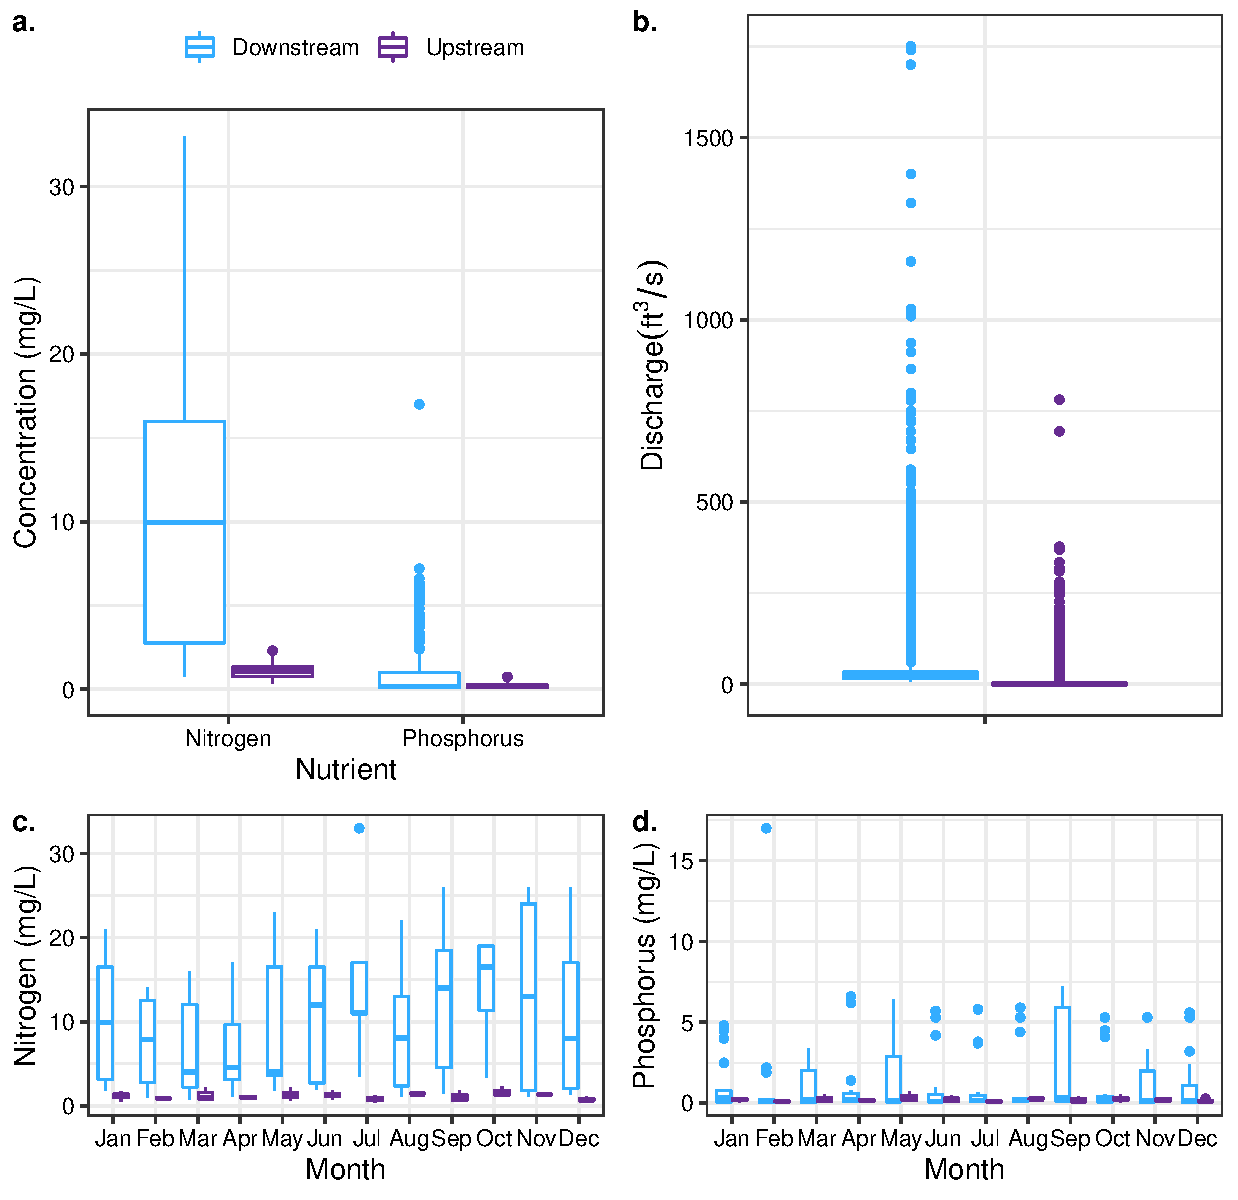
\includegraphics{Landman_ENV872_Project_files/figure-latex/Data Analysis Figure 9-1.pdf}
\caption{Distributions of nutrient concentrations and flow at upstream
and downstream monitoring sites along Ellerbe Creek in North Carolina.
a) Nitrogen and phosphorus concentrations at upstream and downstream
monitoring sites. b) Flow at upstream and downstream monitoring sites.
c) and d) Monthly distributions of nitrogen and phosphorus
concentrations at upstream and downstream monitoring sites.}
\end{figure}

\newpage

\hypertarget{summary-and-conclusions}{%
\section{Summary and Conclusions}\label{summary-and-conclusions}}

It is clear from the results that Ellerbe Creek has high levels of both
phosphorus and nitrogen. While average nitrogen levels are not above EPA
recommendations, the range in nitrogen concentration demonstrates that
at many times throughout the last 30 years, nitrogen concentrations have
been above recommended levels. It was suprising to discover that flow is
a significant predictor of phosphorus but no nitrogran. Furthermore, it
is rare to find a positive relationship between phosphorus and flow and
negative (although not significant) relationship between nitrogen and
flow. Moatar et al. (2017), analyzed concentration versus flow plots,
similar to those presented here and highlighed the interplay of
biological and hydrological dynamics. They outline that a positive
relationship between flow and concentration during low flow events shows
biogeochemical retnetion removal and during a high flow it shows
hydrological export. A negative correlation between concentration and
dischage at both low and high flow levels shows hydrological dilution.
Similar to the pattern observed in Ellerbe Creek, they found higher
levels of NO3\textsuperscript{-} during low flows in 71\% of the
catchments they studied in France. Their findings also show that efforts
to reduce nutrient loading decreased phosphorus concentration, altering
the concentration discharge curve for phosphorus, while nitrate
continued to increase (Moatar et al., 2017). Since Ellerbe Creek and
Falls Lake were listed on the state's impaired water bodies, there have
been efforts throughout the city of Durham and the entire watershed to
prevent nutrient runoff. Throughout the study period land along the
creek has been restored to increase buffering and prevent nutrient
runoff and creek smart installations have reduced runoff from people's
yards. These efforts could influence the relationship between nutrients
and discharge.

The statistical analyses performed show there is a significant
difference between nitrogen at downstream locations and upstream
locations. This is valauble information because Ellerbe Creek discharges
into Falls Lake and therefore higher nitrogen concentrations downstream
can have implications for the water quality in Falls Lake. Ellerbe Creek
runs through an extremely populated area with many potential sources of
nitrogen including agricultural runoff and domestic wastewater.
Additionally, analysis showed a significant difference between discharge
at each location, which could indicate that water is entering the creek
through runoff. Further studies should be done to assess land use and
land cover between upstream and downstream locations to determine the
sources of nitrogen and phosphorus. Additionally, while month is not a
predictor for nitrogen or phosphorus levels, other factors such as
precipitation, temperature, and other contaminents should be examined to
determine all the potential predictors of nutrient levels.

\newpage

\hypertarget{references}{%
\section{References}\label{references}}

City of Durham (2018), Ellerbe Creek Watershed.
\href{https://durhamnc.gov/711/Ellerbe-Creek-Watershed}{link}

City of Durham (2020), Falls Lake.
\href{https://durhamnc.gov/716/Falls-Lake}{link}

Environmental Protection Agency (2013), Total Nitrogen
\href{www.epa.gov/sites/production/files/2015-09/documents/totalnitrogen.pdf}{link}

Environmental Protection Agency (2013), Total Phosphorus
\href{https://www.epa.gov/sites/production/files/2015-09/documents/totalphosphorus.pdf}{link}

North Carolina Department of Environmental Quality (2009), Neuse River
Basinwide Water Quality Plan.
\href{https://deq.nc.gov/about/divisions/water-resources/planning/basin-planning/water-resource-plans/neuse-2009}{link}

Moatar, F., B. W. Abbott, C. Minaudo,F. Curie, and G. Pinay (2017),
Elementalproperties, hydrology, and biologyinteract to shape
concentration-discharge curves for carbon, nutrients,sediment, and major
ions, WaterResour. Res., 53, 1270--1287,\url{doi:10.1002/2016WR019635}


\end{document}
